\section{Motivation}
\frame{\sectionpage}

\begin{frame}{Value of Browser Exploit Chains}
    Web Browsers are some of the highest priority targets for hackers! According to Zerodium, 
    \begin{columns}
        \begin{column}{0.4\textwidth}
            \begin{block}{Desktop Systems}
                \begin{enumerate}
                    \item Windows 0-Click RCE     (\$1m)
                    \item Chrome RCE+LPE          (\$500k)
                    \item MS Outlook/Office RCE (\$250k)
                    \item Linux LPE               (\$50k)
                \end{enumerate}
            \end{block}
        \end{column}
        \begin{column}{0.4\textwidth}
            \begin{block}{Mobile Systems}
                \begin{enumerate}
                    \item Android/iOS Full-chain    (\$2m+)
                    \item WhatsApp 0-click (\$1.5m)
                    \item Chrome RCE+LPE            (\$500k)
                    \item Baseband RCE+LPE          (\$200k)
                \end{enumerate}
            \end{block}
        \end{column}
    \end{columns}
    \note{
        \begin{itemize}
            \item Note, prices last updated April 2024.
            \item Estimated black market prices are about 10x what Zerodium pays.
            \item Other browsers payout at about 100k on Desktop. Safari pays out highly on Mobile at 500k.
            \item In reality, there are only 3 engines that have payouts: Mozilla Spidermonkey, Apple Webkit, and Chrome V8.
        \end{itemize}
    }
\end{frame}

\begin{frame}{APT Orchestration of Browser Exploit Chains}
    \begin{itemize}
        \item Browser exploit chains, due to their complexity, are mainly employed by nation states. 
        Nation state actors without advanced cyber tend to use commercial spyware vendors.
    \end{itemize}
    \begin{block}{1-Click Phishing Campaigns}
        In classical phishing campaigns, distributed links lead to exploitation via a crafted webpage.
    \end{block}
    \begin{block}{0-Click Network Redirection Campaigns}
        These chains use fake networks or compromise public ones to redirect users to malicious sites.
    \end{block}
    \begin{block}{0-Click Man-in-the-Middle Campaigns}
        Plaintext HTTP traffic is modified to redirect to a malicious webpage, often at the ISP level. 
    \end{block} 
    \begin{itemize}
        \item PBS Frontline and Forbidden Films filmed an  \href{https://www.pbs.org/wgbh/frontline/documentary/global-spyware-scandal-exposing-pegasus/}{\color{pink}{excellent documentary}} on NSO Group. 
    \end{itemize}
    \note{
        \begin{itemize}
            \item Most of these attack patterns were observed empirically by Google Threat Analysis Group.
            \item Victims of browser exploit chains tend to be prominent political figures, journalists, etc.
            \item "Advanced cyber capable nation states" are mainly identified as
            \begin{enumerate}
                \item China
                \item Five Eyes "United States, Australia, UK, New Zealand, and Canada" 
                \item Israel
                \item Russia
                \item CISA also cites North Korea and Iran, but most evidence suggests these actors are not quite as mature
            \end{enumerate}
        \end{itemize}
    }
\end{frame}

\begin{frame}{V8 in Browser Exploit Chains}
    \begin{columns}
        \begin{column}{0.30\textwidth}
            It's easy as 1-2-3!
            \begin{enumerate}
                \item Remote code execution
                \item Sandbox escape
                \item Privilege Escalation
            \end{enumerate}
        \end{column}
        \begin{column}{0.70\textwidth}
            \begin{figure}
                \centering
                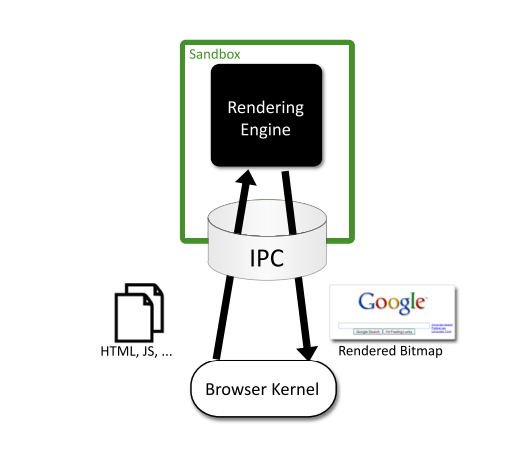
\includegraphics[width=0.66\textwidth]{images/chrome-security-model.PNG}
                \caption{\href{https://seclab.stanford.edu/websec/chromium/chromium-security-architecture.pdf}{\footnotesize{\color{pink}{The Security Architecture of the Chromium Browser}}, Stanford Seclab.}}
                \label{fig:chrome-security-model}
            \end{figure}
        \end{column}
    \end{columns}
    \note{\begin{itemize}
        \item The JavaScript engine is by far the most rich attack surface within the renderer (Rendering Engine).
        \item Historically, a sandbox escape occurs using the IPC channel (Mojo).
        \item However, in recent years, this has moved into attacks on the GPU process (Skia) and other more privileged processes in Chrome.
        \item In rare cases, the renderer may be able to directly exploit the kernel, and skip the SBE. This was the case in the famous BadBinder exploit recovered by Maddie Stone.
        \item It's also possible to bypass the renderer with a powerful vulnerability, these are marked as "Critical" in Chrome's security bulletins. 
        \item Some exploit chains as few as 2 vulnerabilities, most contain 3-5. 
    \end{itemize}}
\end{frame}

\begin{frame}{V8 is Everywhere!}
    \begin{columns}
        \begin{column}{0.33\textwidth}
            (Blink)
            \begin{enumerate}
                \item Google Chrome
                \item Adobe CC
                \item Steam client
                \item Android Webview
                \item Unreal Engine
                \item Matlab
                \item Power BI
                \item Spotify Client
            \end{enumerate}
        \end{column}
        \begin{column}{0.34\textwidth}
            (Node.js)
            \begin{enumerate}
                \item Amazon Web Services
                \item Netflix
                \item PayPal 
                \item Visual Studio Code
                \item Electron framework
                \item Discord
                \item GitHub Desktop
                \item WordPress
            \end{enumerate}
        \end{column}
        \begin{column}{0.33\textwidth}
            (Qt 5)
            \begin{enumerate}
                \item KDE
                \item VirtualBox
                \item Wireshark
                \item Photoshop
                \item Valve's Source 2
                \item Telegram
                \item Tesla Model S UI
                \item Dolphin Emulator
            \end{enumerate}
        \end{column}
    \end{columns}
    \note{
        \begin{itemize}
            \item Blink is the renderer inside Chromium, that handles most of the document object model.
            \item Node.js is a framework that extends JavaScript to handle most OS-level programming. (also electron). 
            \item Qt5 is a graphics rendering engine that extends its graphical functionality using JavaScript.
            \item In many cases, there can be a significant patch gap between vulnerabilities in V8 mainline and their services!
        \end{itemize}
    }
\end{frame}